\section{Experiments}\label{sec:testing}
In this section we are going to perform a number of experiments on our 456 GB dataset of 2 million matches. Firstly we are going to perform some initial experiments on a single computer, to get an idea of the strength of features in \Cref{sec:initialtest}. In \Cref{sec:clustertest}, we will present the experiments that have been running on the cluster. Lastly in \Cref{sub:knowledge} we present a list of the knowledge which can be extracted from our results. All following experiments will be performed using a split of $\frac{2}{3}$ for training set and $\frac{1}{3}$ for testing set. 

\subsection{Initial experimentation}\label{sec:initialtest}
In this section we will present experiments which have been run on a smaller dataset, to get a quick overview of the strength of features. These experiments are used to find the settings, which the cluster should be run with when the final cluster experiments will be performed. 


\subsubsection{Feature symmetry experiment}
In \Cref{sec:representationoffeatures} we represented four different ways of representing features, to capture a possible symmetry in the choice of champions and the layout of the map. In this section we test each representation by training a classifier using logistic regression using the given representation of features. The experiment was performed on a test set of 10,000 matches with training sets of up to 50,000 matches. The result, shown in \Cref{fig:feat-rep}, indicates that method 1 and 4 are very close, but as the binary representation is slightly more accurate than the ternary one the majority of the time, we choose to conduct all the following tests using the binary representation. 

\begin{figure}[!htb]
  \centering
  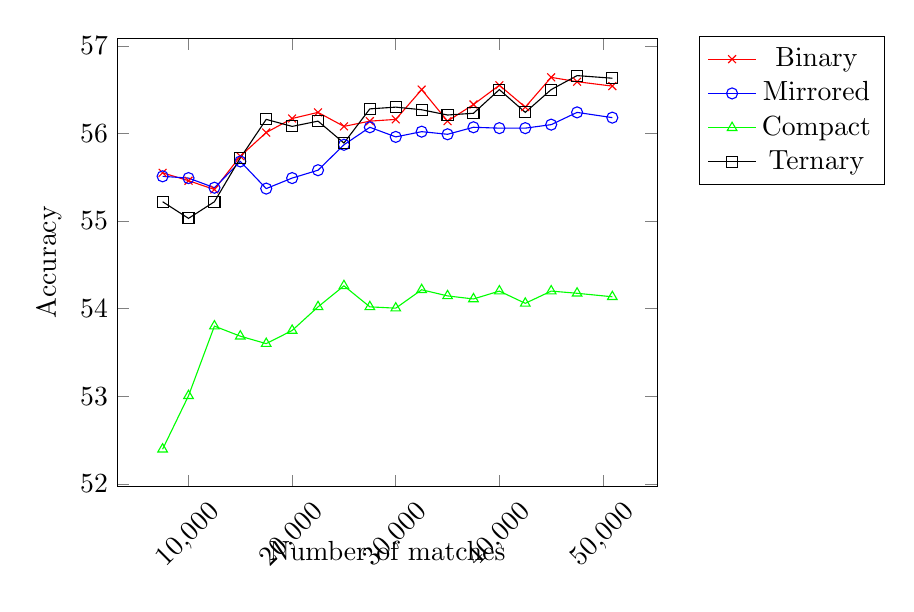
\begin{tikzpicture}[] 
    \begin{axis}[
      xlabel=Number of matches, 
      ylabel=Accuracy,
      xtick={10000,20000,30000,40000,50000},
      xticklabel style={rotate=45,anchor=near xticklabel},
      scaled x ticks=false,
      x label style={at={(axis description cs:0.5,-0.1)},anchor=north},
      legend style={at={(1.25,1.005)},
        anchor=north,legend columns=1},] 
      \addplot[color=red,mark=x] coordinates { 
        (7500, 55.55)
        (10000, 55.46)
        (12500, 55.36)
        (15000, 55.74)
        (17500, 56.01)
        (20000, 56.17)
        (22500, 56.24)
        (25000, 56.08)
        (27500, 56.14)
        (30000, 56.16)
        (32500, 56.50)
        (35000, 56.14)
        (37500, 56.33)
        (40000, 56.55)
        (42500, 56.30)
        (45000, 56.64)
        (47500, 56.59)
        (50901, 56.54)
      };
      \addplot[color=blue,mark=o] coordinates { 
        (7500, 55.51)  
        (10000, 55.49)
        (12500, 55.38)
        (15000, 55.68)
        (17500, 55.37)
        (20000, 55.49)
        (22500, 55.58)
        (25000, 55.87)
        (27500, 56.07)
        (30000, 55.96)
        (32500, 56.02)
        (35000, 55.99)
        (37500, 56.07)
        (40000, 56.06)
        (42500, 56.06)
        (45000, 56.10)
        (47500, 56.24)
        (50901, 56.18)
      };
      \addplot[color=green,mark=triangle] coordinates { 
        (7500, 52.395)  
        (10000, 53.005)
        (12500, 53.80)
        (15000, 53.685)
        (17500, 53.60)
        (20000, 53.75)
        (22500, 54.02)
        (25000, 54.26)
        (27500, 54.02)
        (30000, 54.005)
        (32500, 54.215)
        (35000, 54.145)
        (37500, 54.11)
        (40000, 54.20)
        (42500, 54.06)
        (45000, 54.20)
        (47500, 54.175)
        (50901, 54.135)
      };
      \addplot[color=black,mark=square] coordinates {
        (7500, 55.22)  
        (10000, 55.03)
        (12500, 55.22)
        (15000, 55.72)
        (17500, 56.16)
        (20000, 56.08)
        (22500, 56.14)
        (25000, 55.89)
        (27500, 56.28)
        (30000, 56.30)
        (32500, 56.27)
        (35000, 56.21)
        (37500, 56.23)        
        (40000, 56.50)
        (42500, 56.24)
        (45000, 56.50)
        (47500, 56.66)
        (50901, 56.63)
      };
      \legend{Binary, Mirrored, Compact, Ternary}
    \end{axis} 
  \end{tikzpicture}
  \caption{Test for representation of features}\label{fig:feat-rep}
\end{figure}

\subsubsection{Best machine learning technique}
Many different machine learning algorithms exists for learning a classifier. In this experiment, we test eight different classifiers provided by Weka (a machine learning tool from The University of Waikato) to see which one gives the best result for our particular problem. The tested classifiers are naive bayes, hidden naive bayes, logistic regression, neural network, support vector machine(C-SVM), adaboost(using decision stump), Hoeffding Tree, and Decision Stump. All the different methods are run with multiple parameter settings to find the configuration that yields the best result. Note that no parameters are needed for naive bayes, hidden naive bayes and decision stump. For logistic regression, different values of the L2-regularisation parameter has been tested. For C-SVM, different values for the $c$-constant has been used as well as linear, polynomial, radial, and sigmoid kernel methods. For Adaboost, different number of iterations have been used. For neural networks, different number of hidden neurons have been used, always placed in a single hidden layer. For Hoeffding Trees, Weka has 7 different parameters, but only the Hoeffding tie threshold and leaf prediction strategy caused a different accuracy when adjusted.

Using 35000 matches in a 2/3 split of train and evaluation, the best accuracy obtained with each of the methods can be seen in \Cref{fig:besttech}. As seen, SVM and Neural networks got the worst accuracy. Naive bayes, adaboost and Hidden naive bayes all have an accuracy close to 56.5\%, but logistic regression has the best accuracy almost hitting 57\%.
The best parameters of each method was found to be:

\begin{center}
\begin{itemize}
\item SVM: sigmoid kernel function, $c = 1$.
\item Adaboost: 200 iterations
\item Logistic regression: L2-regularisation constant = 0.0016
\item Neural Network: $(\text{attributes} + \text{classes}) / 2$ hidden neurons.
\item Hoeffding Tree: Hoeffding tie threshold: 0.001, leaf prediction strategy: Naive Bayes.
\end{itemize}

\begin{figure}[!htb]
  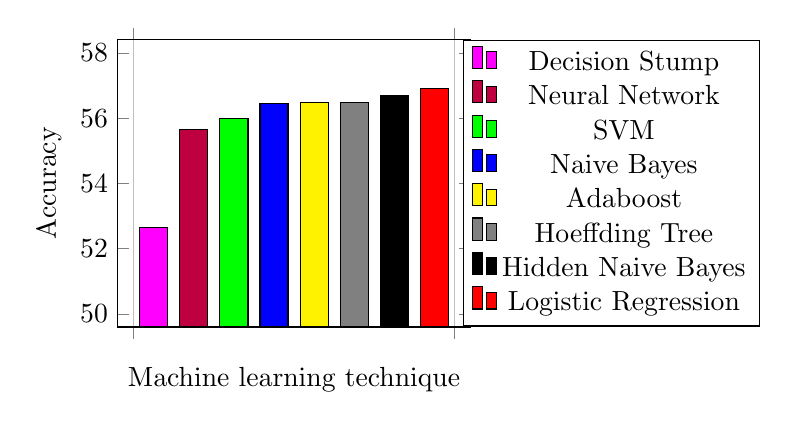
\begin{tikzpicture}
    \begin{axis}[
      %x tick label style={/pgf/number format/1000 sep=},
      xticklabel=\empty,
      ylabel=Accuracy,
      xlabel=Machine learning technique,
      enlargelimits=0.05,
      legend style={at={(1.4,1.0)},
        anchor=north,legend columns=1},
      ybar interval=0.7,
      width=.50\textwidth,
      ymin=50, ymax=58,
      reverse legend,
      ]
      \addplot[fill=red] coordinates {(1,56.916) 
        (0,2)
      };
      \addplot[fill=black] coordinates {(1,56.6807) 
        (0,56.6807)
      };

\addplot[fill=gray] coordinates {(1,56.48)
        (0,0)
      };      
      
      
      \addplot[fill=yellow] coordinates {(1,56.479) 
        (0,2)
      };
      \addplot[fill=blue] coordinates {(1,56.4454) 
        (0,56.4454)
      };
      \addplot[fill=green] coordinates {(1,55.98)
        (0,0)
      };
      \addplot[fill=purple] coordinates {(1,55.6555) 
        (0,0)
      };      
      \addplot[fill=Fuchsia] coordinates {(1,52.64)
        (0,0)
      };
      \legend{Logistic Regression,Hidden Naive Bayes,Hoeffding Tree,Adaboost,Naive Bayes,SVM,Neural Network, Decision Stump}
    \end{axis} 
  \end{tikzpicture}
  \caption{Test of best machine learning technique}\label{fig:besttech}
\end{figure}
\end{center}

\subsubsection{Best features}
\label{sec:best-features}
To get an idea of each type of features impact on our prediction capability, some quick tests are performed using the machine learning tool Weka.
Logistic regression is used as classifier with an L2-regularization parameter of 750. A training set of ranging size is used, up to a total of 50,000 matches, and a test set of 10,000 matches is used for evaluation.
The obtained accuracies can be seen in \Cref{fig:best-feat}.
Interestingly, the baseline where no features are used gives an accuracy of $51.24 \%$, and results in a model that always predicts the blue team to win.
Among the feature types that only consider the rank of players, the $\phi_\text{LANE-RANKS}$ feature did best.
The $\phi_\text{PAIR}$ and $\phi_\text{COUNTER}$ features have not been tested, as they due to their size and density could not be handled in Weka on a machine with 8 GB memory.
Those tests are therefore performed on the cluster, described in \Cref{sec:clustertest}.
When using more types of features at the same time, one may think that the accuracy always improves, but this is however not the case.
If all 3 types of features concerned with player ranks are used, an accuracy of only $56.06 \%$ is achieved compared to $56,39 \%$ when using the $\phi_\text{LANE-RANKS}$ features alone. There is no combination of rank feature types that gives a better accuracy than just using the best of them alone.
However, combining feature types that captures different phenomenons seems to increase the accuracy.
Among the tested feature types, the best feature types to combine has been found to be the $\phi_\text{LANE-RANKS}$ and $\phi_\text{LANE-CHAMPION}$ feature types from which an accuracy of $58.73 \%$ were achieved.


\begin{figure}[!htb]
  \centering
  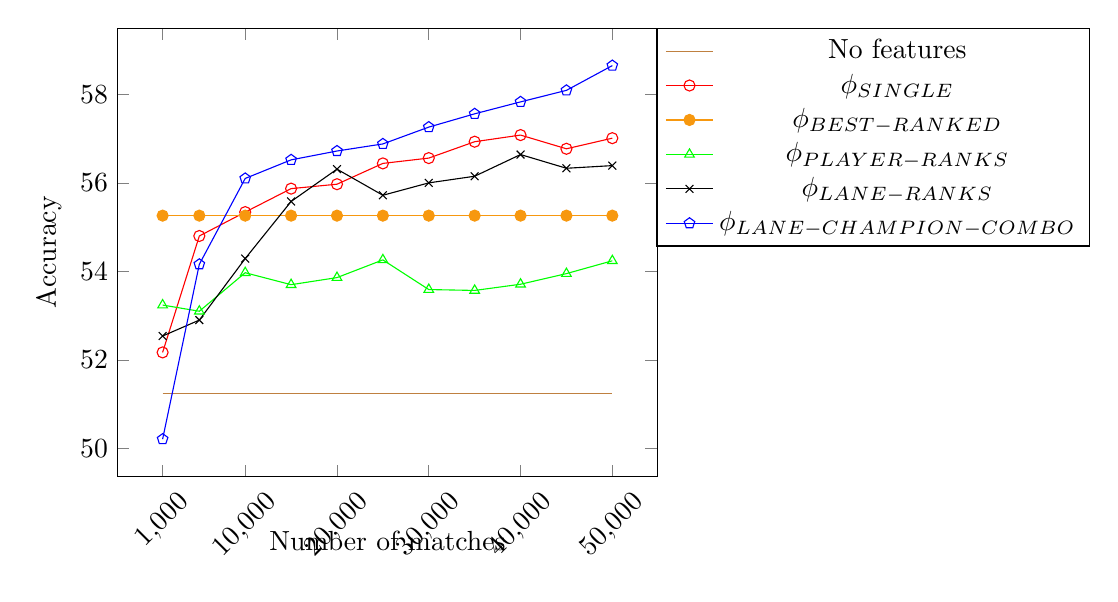
\begin{tikzpicture}[] 
    \begin{axis}[
      xlabel=Number of matches, 
      ylabel=Accuracy,
      xtick={1000,10000,20000,30000,40000,50000},
      xticklabel style={rotate=45,anchor=near xticklabel},
      scaled x ticks=false,
      x label style={at={(axis description cs:0.5,-0.1)},anchor=north},
      legend style={at={(1.4,1.001)},
        anchor=north,legend columns=1},] 
      \addplot[color=brown] coordinates { 
        (1000,51.24)
        (5000,51.24)
        (10000,51.24)
        (15000,51.24)
        (20000,51.24)
        (25000,51.24)
        (30000,51.24)
        (35000,51.24)
        (40000,51.24)
        (45000,51.24)
        (50000,51.24)
      };
      \addplot[color=red,mark=o] coordinates { 
        (1000,52.17)
        (5000,54.8)
        (10000,55.34)
        (15000,55.87)
        (20000,55.97)
        (25000,56.44)
        (30000,56.56)
        (35000,56.93)
        (40000,57.08)
        (45000,56.77)
        (50000,57.01)
      };
      \addplot[color=YellowOrange,mark=*] coordinates { 
        (1000,55.26)
        (5000,55.26)
        (10000,55.26)
        (15000,55.26)
        (20000,55.26)
        (25000,55.26)
        (30000,55.26)
        (35000,55.26)
        (40000,55.26)
        (45000,55.26)
        (50000,55.26)
      };
      \addplot[color=green,mark=triangle] coordinates { 
        (1000,53.24)
        (5000,53.1)
        (10000,53.97)
        (15000,53.7)
        (20000,53.86)
        (25000,54.26)
        (30000,53.59)
        (35000,53.57)
        (40000,53.71)
        (45000,53.95)
        (50000,54.24)
      };
      \addplot[color=black,mark=x] coordinates { 
        (1000,52.54)
        (5000,52.90)
        (10000,54.29)
        (15000,55.58)
        (20000,56.31)
        (25000,55.72)
        (30000,56.00)
        (35000,56.15)
        (40000,56.64)
        (45000,56.33)
        (50000,56.39)
      };
      \addplot[color=blue,mark=pentagon] coordinates { 
        (1000,50.21)
        (5000,54.16)
        (10000,56.10)
        (15000,56.52)
        (20000,56.72)
        (25000,56.88)
        (30000,57.26)
        (35000,57.56)
        (40000,57.83)
        (45000,58.09)
        (50000,58.65)
      };
      \legend{No features,$\phi_\text{SINGLE}$, $\phi_\text{BEST-RANKED}$, $\phi_\text{PLAYER-RANKS}$,$\phi_\text{LANE-RANKS}$,$\phi_\text{LANE-CHAMPION-COMBO}$}
    \end{axis} 
  \end{tikzpicture}
  \caption{Accuracy of features}\label{fig:best-feat}
\end{figure}